\documentclass[11pt,a4paper,twoside]{article}%
\usepackage{amsmath}
\usepackage{amsfonts}

\usepackage{color}
\usepackage{amssymb}
\usepackage{graphicx}%
\setcounter{MaxMatrixCols}{30}
%TCIDATA{OutputFilter=latex2.dll}
%TCIDATA{Version=5.50.0.2953}
%TCIDATA{CSTFile=40 LaTeX article.cst}
%TCIDATA{Created=Thursday, December 26, 2013 11:29:10}
%TCIDATA{LastRevised=Thursday, January 05, 2017 16:30:54}
%TCIDATA{<META NAME="GraphicsSave" CONTENT="32">}
%TCIDATA{<META NAME="SaveForMode" CONTENT="1">}
%TCIDATA{BibliographyScheme=Manual}
%TCIDATA{<META NAME="DocumentShell" CONTENT="Standard LaTeX\Blank - Standard LaTeX Article">}
%BeginMSIPreambleData
\providecommand{\U}[1]{\protect\rule{.1in}{.1in}}
%EndMSIPreambleData
\newtheorem{theorem}{Theorem}
\newtheorem{acknowledgement}[theorem]{Acknowledgement}
\newtheorem{algorithm}[theorem]{Algorithm}
\newtheorem{axiom}[theorem]{Axiom}
\newtheorem{case}[theorem]{Case}
\newtheorem{claim}[theorem]{Claim}
\newtheorem{conclusion}[theorem]{Conclusion}
\newtheorem{condition}[theorem]{Condition}
\newtheorem{conjecture}[theorem]{Conjecture}
\newtheorem{corollary}[theorem]{Corollary}
\newtheorem{criterion}[theorem]{Criterion}
\newtheorem{definition}[theorem]{Definition}
\newtheorem{example}[theorem]{Example}
\newtheorem{exercise}[theorem]{Exercise}
\newtheorem{lemma}[theorem]{Lemma}
\newtheorem{notation}[theorem]{Notation}
\newtheorem{problem}[theorem]{Problem}
\newtheorem{proposition}[theorem]{Proposition}
\newtheorem{remark}[theorem]{Remark}
\newtheorem{solution}[theorem]{Solution}
\newtheorem{summary}[theorem]{Summary}
\newenvironment{proof}[1][Proof]{\noindent\textbf{#1.} }{\ \rule{0.5em}{0.5em}}
\topmargin -0.7in
\oddsidemargin -0.30in
\evensidemargin -0.7in
\textwidth 7.3in
\textheight 9.5in
\begin{document}

\begin{center}
\textbf{\textsf{Estad\'{\i}stica (Qu\'{\i}mica) }}

\textbf{Pr\'{a}ctica 5 - Estimaci\'{o}n - Intervalos de Confianza\vspace
{-0.1in}}
\end{center}

Comentario: En todos los ejercicios propuestos

\begin{enumerate}
\item[a)] defina las variables aleatorias y los par\'{a}metros involucrados.

\item[b)] de ser posible indique:

\begin{enumerate}
\item[i.] la distribuci\'{o}n de las variables aleatorias

\item[ii.] el significado intuitivo de los par\'{a}metros.
\end{enumerate}

\item[c)] compare los resultados de hacer las cuentas a mano con las salidas
obtenidas con el R, de manera de chequear las primeras y aprender a usar las
segundas, en aquellos ejercicios en los que ambas cosas sean posibles.
\end{enumerate}

\begin{enumerate}

\item Considere el ejercicio 4 de la Pr\'{a}ctica de Estad\'{\i}stica Descriptiva.

\begin{enumerate}
\item Usando las medias y desviaciones est\'{a}ndar calculadas en R,
calcule un IC del 95\% para la media de las mediciones hechas por cada uno de
los grupos. \textquestiondown Los intervalos obtenidos tienen nivel de
confianza exacto o aproximado? Para responder esta pregunta,
recuerde lo realizado al analizar los datos en la pr\'{a}ctica de descriptiva.

\item Observe que R tambi\'{e}n puede calcular
autom\'{a}ticamente los ICs del inciso anterior. Considere la instrucci\'{o}n:%
\[
\text{\texttt{t.test(GRUPO1,alternative= "two.sided")}}%
\]

\item \textquestiondown Es razonable pensar que ambos grupos de estudiantes
est\'{a}n midiendo la concentraci\'{o}n de ion nitrato sin sesgo? En caso
contrario, \textquestiondown puede saberse si uno solo o ambos grupos hacen
mediciones sesgadas?
\end{enumerate}

\item Ciudad G\'{o}tica tiene numerosas casas alquiladas. Para realizar un
estudio se eligen 400 al azar y se averigua el alquiler que pagaron sus
ocupantes el mes anterior, resultando un promedio muestral $\overline
{x}=\$184$ y un desv\'{\i}o est\'{a}ndar muestral $s=\$80$. Se dibuja un
histograma con los alquileres registrados en la muestra y se ve que no sigue
la curva normal.

\begin{enumerate}
\item Si es posible, halle un intervalo de confianza del 68\% aproximadamente
para el alquiler medio de las casas de alquiler ocupadas en Ciudad G\'{o}tica.
Si no es posible, justifique.

\item Indique si es verdadero o falso: Para alrededor del 68\% del total de
casas de alquiler ocupadas en la ciudad, el alquiler fue de entre \$180 y \$188.
\end{enumerate}

\item Una balanza comete errores aleatorios que siguen la densidad que se
muestra en el gr\'{a}fico:%

\begin{center}
	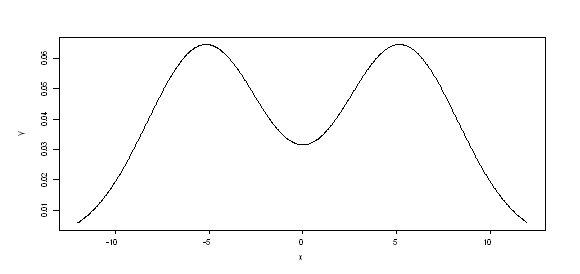
\includegraphics[width=\textwidth]{densidadpracticaIC.jpg}
\end{center}

La esperanza de esta densidad es 0 microgramos y su desviaci\'{o}n
est\'{a}ndar es 6 microgramos. Se hacen 4 mediciones de un peso y se requiere
un intervalo de confianza (exacto o aproximado) para el peso verdadero.

\begin{enumerate}
\item Para hallar el intervalo de confianza, \textquestiondown puede usarse la
curva normal? \textquestiondown Y la $t$ de Student? Justifique.

\item \'{I}dem con 100 mediciones. D\'{e} el intervalo correspondiente para un
nivel del 95\% e indique si es exacto o aproximado.

\item Se hacen 100 mediciones, en 57 de las cuales se comete un error
positivo. Hallar un intervalo de confianza de nivel 95\% aproximadamente para
la proporci\'{o}n de mediciones en las que se cometen errores positivos.
Investigar las siguientes instrucciones de R, y compararlas con la
resoluci\'{o}n a mano del ejercicio.
\begin{gather*}
\text{\texttt{prop.test(x = 57,n = 100,correct=TRUE)}}\\
\text{\texttt{prop.test(x = 57,n = 100,correct=FALSE)}}\\
\text{\texttt{binom.test(x = 57,n = 100)}}%
\end{gather*}

\end{enumerate}

\item Para un estudio de mercado 277 personas degustan un nuevo licor y
69 de ellas desaprueban el nuevo sabor. Construya un intervalo de
aproximadamente 95\% de confianza para la verdadera proporci\'{o}n poblacional
$p$ de personas que aprueban el nuevo licor.

\item Un fabricante asegura a una compa\~{n}\'{\i}a (que le compra un
producto en forma regular) que el porcentaje de productos defectuosos no es
mayor del 5\%. La compa\~{n}\'{\i}a decide comprobar la afirmaci\'{o}n del
comerciante seleccionando al azar de su inventario 200 unidades de este
producto y prob\'{a}ndolas. En la muestra encuentran 19 unidades defectuosas.

\begin{enumerate}
\item Construya un intervalo del 95\% aproximadamente de confianza para la
verdadera proporci\'{o}n de unidades defectuosas.

\item \textquestiondown Tiene razones la compa\~{n}\'{\i}a para sospechar de
la afirmaci\'{o}n del fabricante? Justifique.
\end{enumerate}


\item Se desea construir un intervalo de confianza para la media $\mu$
del puntaje de cierta prueba de lectura dise\~{n}ada para los alumnos de
tercer grado de la ciudad de Buenos Aires. Supongamos que, de estudios
anteriores, se puede inferir que el desv\'{\i}o est\'{a}ndar poblacional es
$\sigma=12.$

\begin{enumerate}
\item Se extrae una muestra al azar de $100$ ni\~{n}os de tercer grado de la
ciudad de Buenos Aires, a los que se les toma la prueba. Calcule la longitud
del intervalo de confianza de nivel 95\%\ basado en dicha muestra. El
intervalo de confianza, \textquestiondown es exacto o aproximado?
\textquestiondown Que hip\'{o}tesis deben satisfacer las variables involucradas?

\item \'{I}dem (a) pero si el presupuesto permitiese s\'{o}lo evaluar a 10 ni\~{n}os.

\item Halle el menor valor de $n$ para el cual se satisface el requerimiento
de los investigadores de obtener un intervalo del 95\% de confianza con una
longitud de a lo sumo 2. Especifique los supuestos utilizados.
\end{enumerate}

\item En un debate sobre contaminaci\'{o}n ambiental, se est\'{a}
evaluando la concentraci\'{o}n de mon\'{o}xido de carbono en las esquinas de
la ciudad en los momentos de mayor tr\'{a}fico (los viernes a la tarde).
Interesa estimar $p$, la proporci\'{o}n de esquinas que presentan valores de
mon\'{o}xido inferiores a 12 ppm (partes por mill\'{o}n). Para ello, se
recolecta una muestra de 120 valores correspondientes al nivel de mon\'{o}xido
de carbono en esquinas de la ciudad aleatoriamente elegidas un viernes a la
tarde. Los datos obtenidos se representan en el siguiente histograma de
densidad.%

\begin{center}
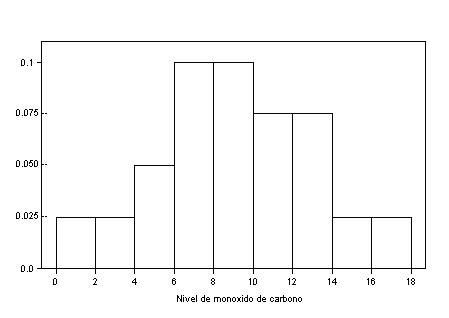
\includegraphics[scale=1]{histogramamonoxidopracticaIC.jpg}
\end{center}


\begin{enumerate}
\item En base a ellos, la estimaci\'{o}n de $p$ resulta ser .........................

\item Para completar el an\'{a}lisis de los datos del \'{\i}tem anterior se
decide calcular un intervalo de confianza de nivel aproximado 0.95 para $p$.
Calc\'ulelo, y brinde los extremos num\'{e}ricos de dicho intervalo: (....................,..........................).
\end{enumerate}

\item Considere el ejercicio 6 de la Pr\'{a}ctica de Estad\'{\i}stica
Descriptiva. Trabajaremos con las nubes Tratadas.

\begin{enumerate}
\item \textquestiondown Puede calcular un intervalo de confianza de nivel 0.95
(exacto o aproximado) para la cantidad esperada de agua ca\'{\i}da de una nube
tratada con un bombardeo de \'{a}tomos? Para responder este \'{\i}tem,
recuerde lo realizado al analizar los datos en la pr\'{a}ctica de descriptiva.

\item \textquestiondown Puede calcular un intervalo de confianza de nivel 0.95
para el valor esperado del logaritmo de la cantidad de agua ca\'{\i}da de una
nube tratada con un bombardeo de \'{a}tomos? Resuelva usando R. A partir
del intervalo calculado, \textquestiondown puede ahora responder positivamente
al \'{\i}tem (a)?
\end{enumerate}

\item En un estudio se le pregunta a un grupo de personas  si est\'a de acuerdo con la frase \textit{ existe un \'unico verdadero amor en la vida}. Se entrevista a 2625 individos;
372 de los 1213 hombres est\'an  de acuerdo con la frase mientras que 363 de las 1412 mujeres concuerdan con el enunciado. Determine si estos datos muestran diferencia entre la opini\'on, a favor de la afirmaci\'on, de hombres y mujeres. 


\item Un estudio examina los efectos del chocolate a partir de los vasos sangu\'ineos de personas sanas. En el estudio aleatorizado, 31 personas recibieron 46 gramos de chocolate negro (que es naturalmente rico en flavonoides) todos los d\'ias durante dos semanas (grupo tratados). 
Por otra parte,   30 personas (grupo control) recibieron un placebo que consiste en chocolate negro con bajo contenido en flavonoides. A los participantes se les midi\'o su salud vascular (por medio de dilataci\'on mediada por flujo) antes y despu\'es de las dos semanas de estudio. Para el grupo que recibi\'o el buen chocolate negro, el promedio de las diferencias (despu\'es-antes) de la dilataci\'on medida fue de 1,3, con una desviaci\'on est\'andar de 2,32. El  grupo control tuvo un cambio promedio de −0,96 (despu\'es-antes) con una desviaci\'on est\'andar de 1,58. 
\begin{enumerate}
	\item Identifique c\'uales son las variables de involucradas en el problema y el par\'ametro de inter\'es. 
\item Calcule un intervalo de confianza asint\'otico estimado del $95\%$ para el par\'ametro de inter\'es.  Interprete.
\item \textquestiondown Es posible que no haya ``diferencia alguna" entre los dos tipos de chocolate? Justifique su respuesta usando el intervalo de confianza encontrado en el \'item anterior. 
\end{enumerate}


\end{enumerate}


\end{document}